\documentclass[parskip=half,DIV=16]{scrartcl}

\title{Lab assignment 3}
\subtitle{ATM S 544}
\author{Dominik Stiller}
\date{\today}

\usepackage[english]{babel}
\usepackage[utf8]{inputenc}
\usepackage{siunitx,amsmath,physics}
\usepackage{caption,subcaption,graphicx,csquotes,xcolor}
\usepackage{booktabs}
\usepackage{placeins}
\usepackage[
	backend=biber,
	bibwarn=true,
	bibencoding=utf8,
	sortlocale=en_US,
	url=false,
	style=apa,
	isbn=false
]{biblatex}

\definecolor{uw-purple}{RGB}{51, 0, 111}

\usepackage{hyperref}
\hypersetup{
	% hidelinks,
	colorlinks=true,
	linkcolor=black,
	citecolor=black,
	urlcolor=uw-purple
}

\usepackage{doi}
\usepackage{nomencl}
\makenomenclature
\usepackage[noabbrev,capitalise]{cleveref}
\usepackage[acronym,nonumberlist,nopostdot,nogroupskip]{glossaries}
\usepackage[
	outputdir=build,
]{minted}
\setminted{
	linenos,
	tabsize=4,
	fontsize=\small,
}
\newmintinline{python}{}

\usepackage{lmodern}
\usepackage[T1]{fontenc}
\usepackage{inconsolata}
\usepackage{tikz}

\newcommand{\result}[1]{\colorbox{uw-purple}{\textcolor{white}{#1}}}

\setlength{\nomlabelwidth}{1.5cm}
\setlength{\nomitemsep}{-\parsep}
\newcommand{\nomunit}[1]{%
\renewcommand{\nomentryend}{\hspace*{\fill}\si{#1}}}

\sisetup{per-mode=symbol}
\AtBeginDocument{\RenewCommandCopy\qty\SI}

\DeclareGraphicsRule{.ai}{pdf}{.ai}{}

\addbibresource{bibliography.bib}



\begin{document}

\maketitle




\section{Single scalar observation for same point}

\begin{figure}[h]
    \centering
 
    \begin{subfigure}[c]{\textwidth}
       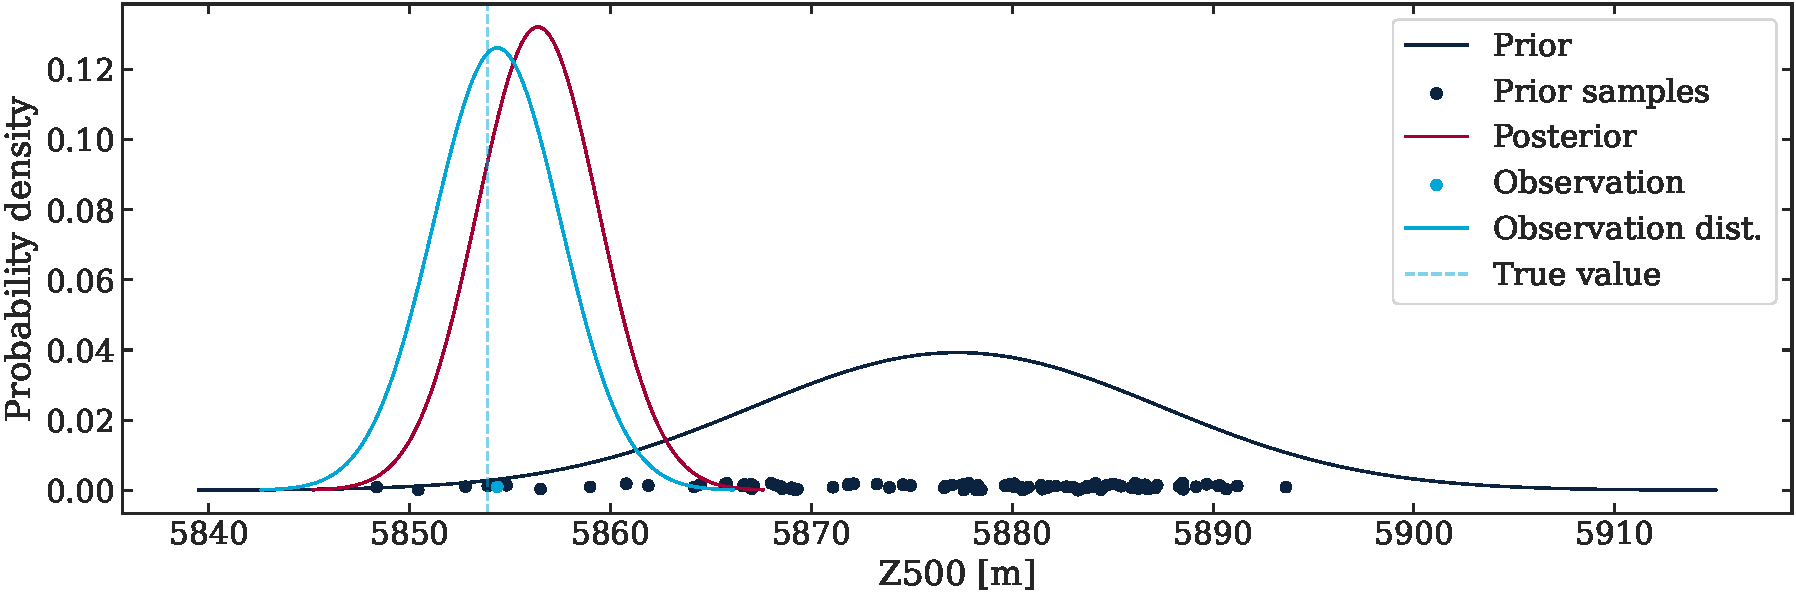
\includegraphics[width=\textwidth]{figures/single_point1.pdf}
       \subcaption{Point 1 (\ang{40} N)}
    \end{subfigure}
     
    \bigskip
     
    \begin{subfigure}[c]{\textwidth}
       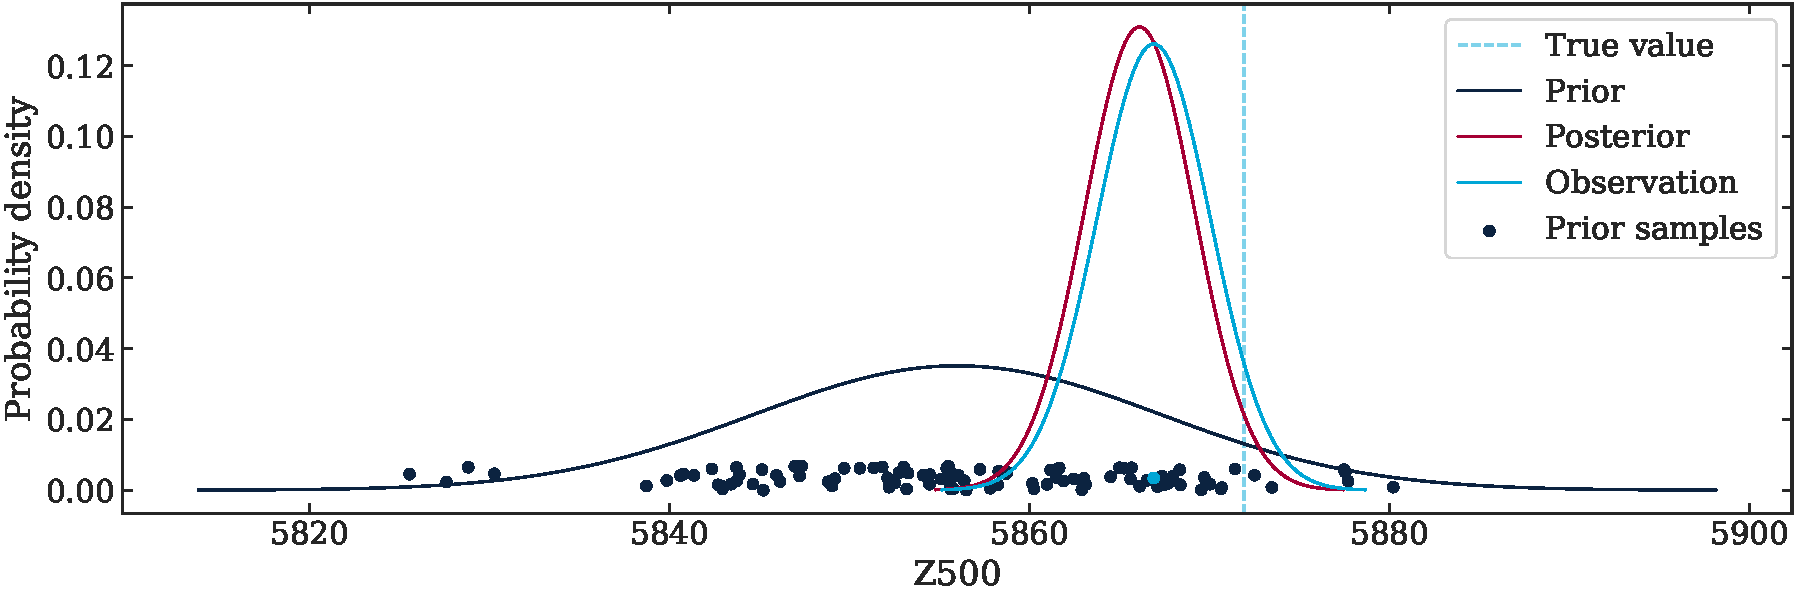
\includegraphics[width=\textwidth]{figures/single_point2.pdf}
       \subcaption{Point 2 (\ang{20} N)}
      \label{fig:single-scalar-2}
    \end{subfigure}
 
    \caption{Assimilation of a single scalar observation.}
 \end{figure}

 Both cases are essentially identical up to the observation sample and the mean. The small variance of the observation relative to the prior pulls the posterior close towards the observation. The posterior is sharper than either prior or observation, indicating the gain in information due to assimilation.

 The observation does not have to align with the true value, which is particularly obvious in \cref{fig:single-scalar-2}. More observations would be necessary to approach the true value.




\section{Multiple scalar observations for same point}

\begin{figure}[H]
   \centering

   \begin{subfigure}[c]{\textwidth}
      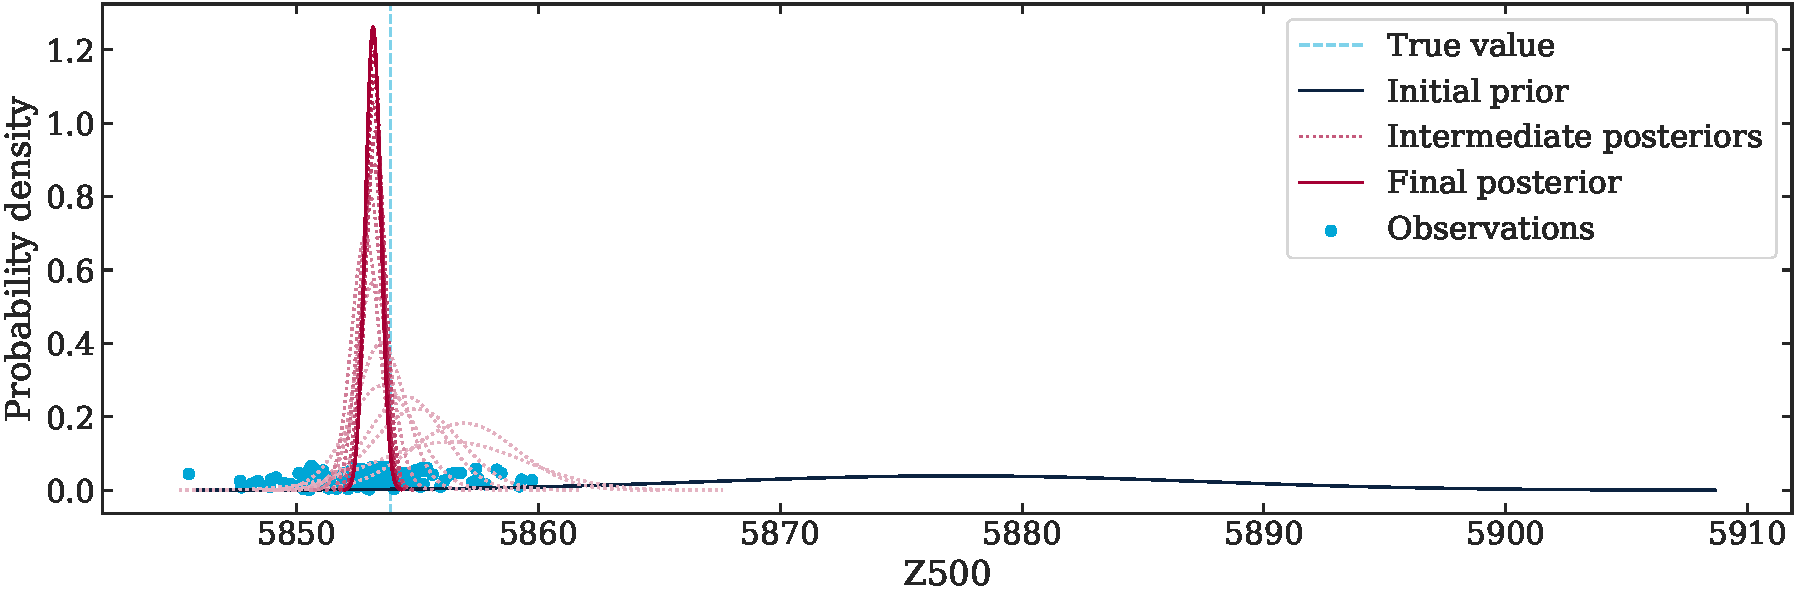
\includegraphics[width=\textwidth]{figures/multiple_point1_var10.pdf}
      \subcaption{Point 1 (\ang{40} N)}
   \end{subfigure}
   
   \bigskip
   
   \begin{subfigure}[c]{\textwidth}
      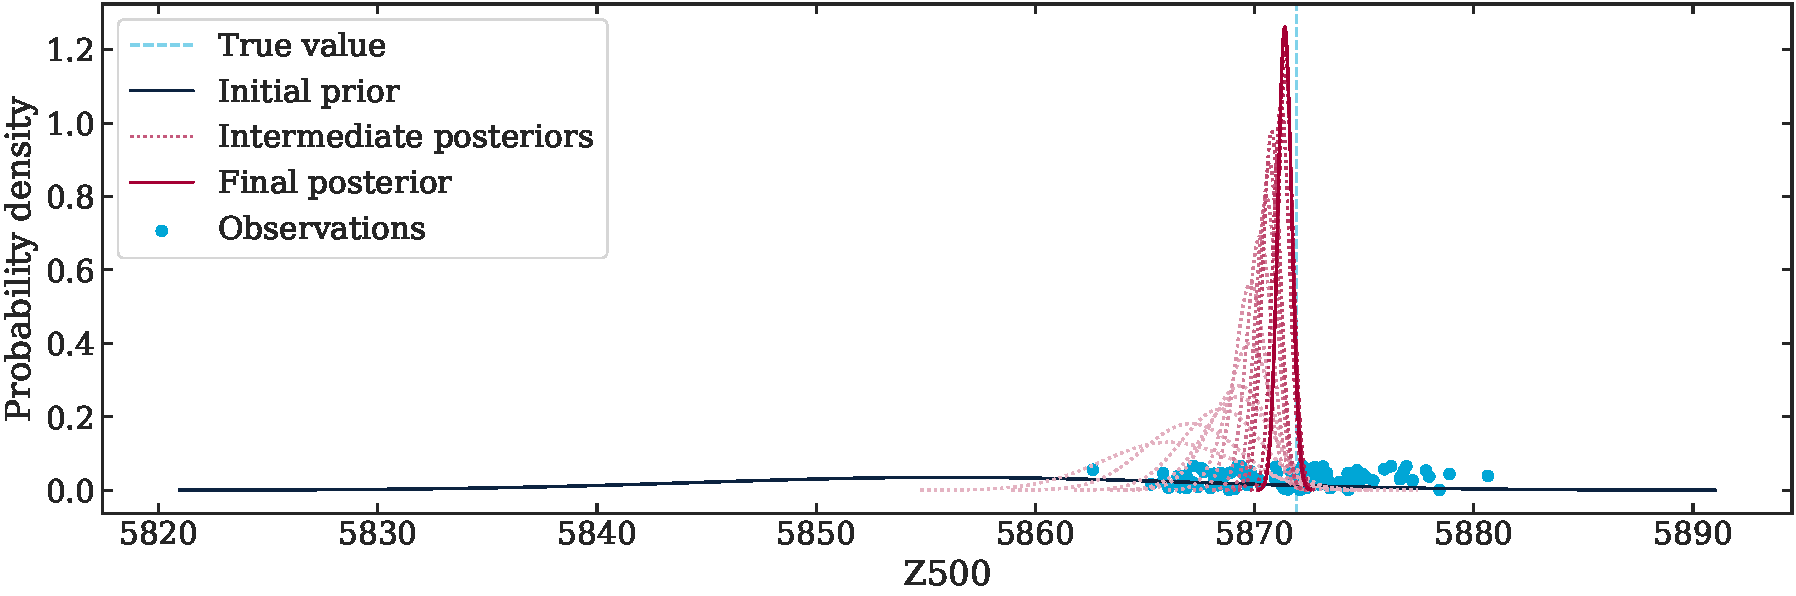
\includegraphics[width=\textwidth]{figures/multiple_point2_var10.pdf}
      \subcaption{Point 2 (\ang{20} N)}
   \end{subfigure}
   
   \caption{Assimilation of 100 scalar observations ($\sigma_y^2 = \qty{10}{m^2}$). The first 5 posteriors are included to show the rapid convergence, only afterwards does the plot switch to every 10 observations.}
\end{figure}

With every observation assimilated, the posterior becomes sharper and its mean converges to the observation mean (i.e., the prior loses relevance). For 100 observations, the observation sample mean is still distinct from the true observation (population) mean. For 1000 observations, they essentially collapse.

After assimilating 100 observations and repeating the process 100 times, the final error variance of the mean is \result{0.10}, as is the mean variance of the posterior. This holds for both points. The ensemble appears well-calibrated and the posterior variance approximates the error variance well. In reality the error variance cannot be known directly since we do not have access to the truth.

I am surprised about the correspondence between posterior variance and error variance. Rather, I would have expected the posterior variance to approximate the mean squared error (i.e., a metric of the \emph{value} of the error rather than its \emph{variability}, since the error already measures a deviation from the mean). Both seem to converge to the same value, however, for many observations, which may or may not be a coincidence.




\subsection{Evolution of prior error, posterior error and posterior variance}

\begin{figure}[H]
   \centering
   
   \begin{subfigure}[c]{\textwidth}
      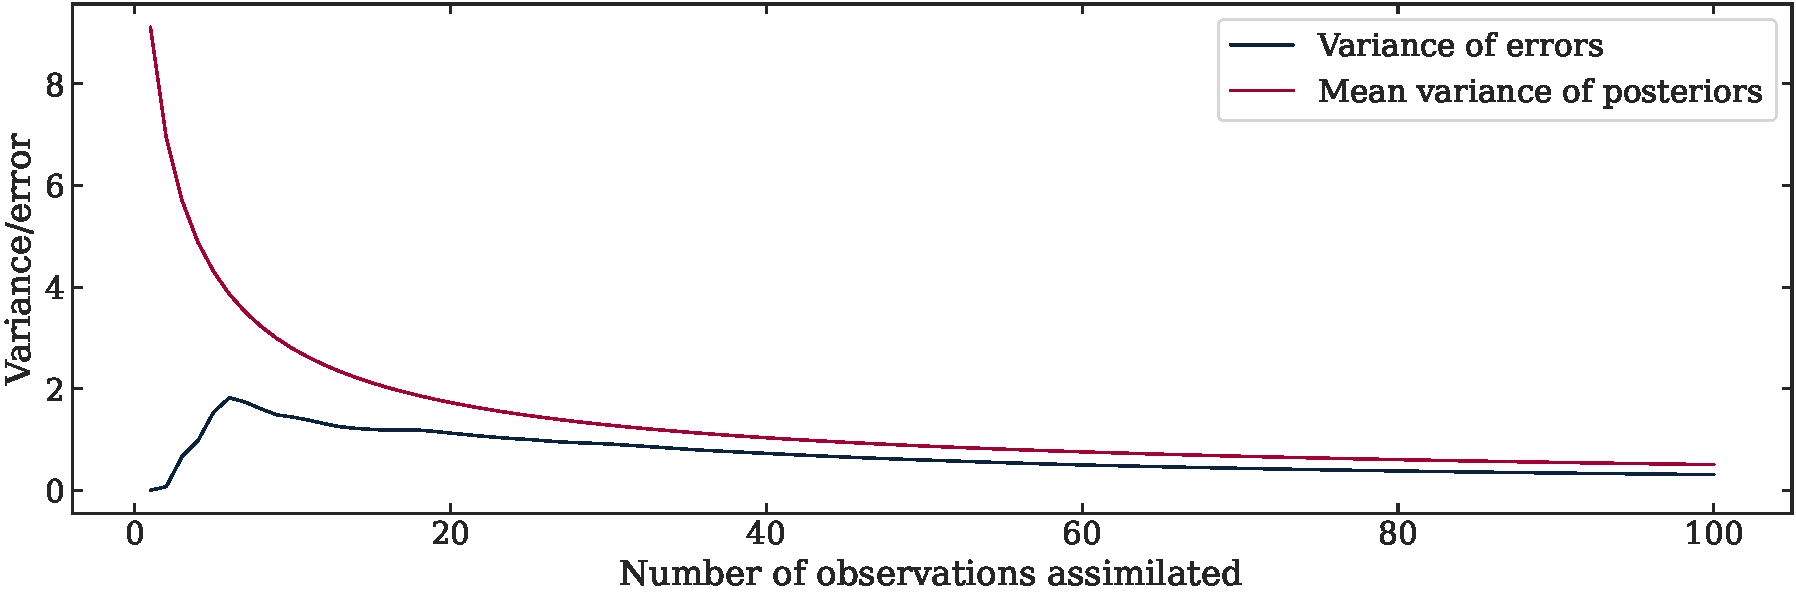
\includegraphics[width=\textwidth]{figures/stats_point1_var10.pdf}
      \subcaption{$\sigma_y^2 = \qty{10}{m^2}$}
   \end{subfigure}
   
   \bigskip
   
   \begin{subfigure}[c]{\textwidth}
      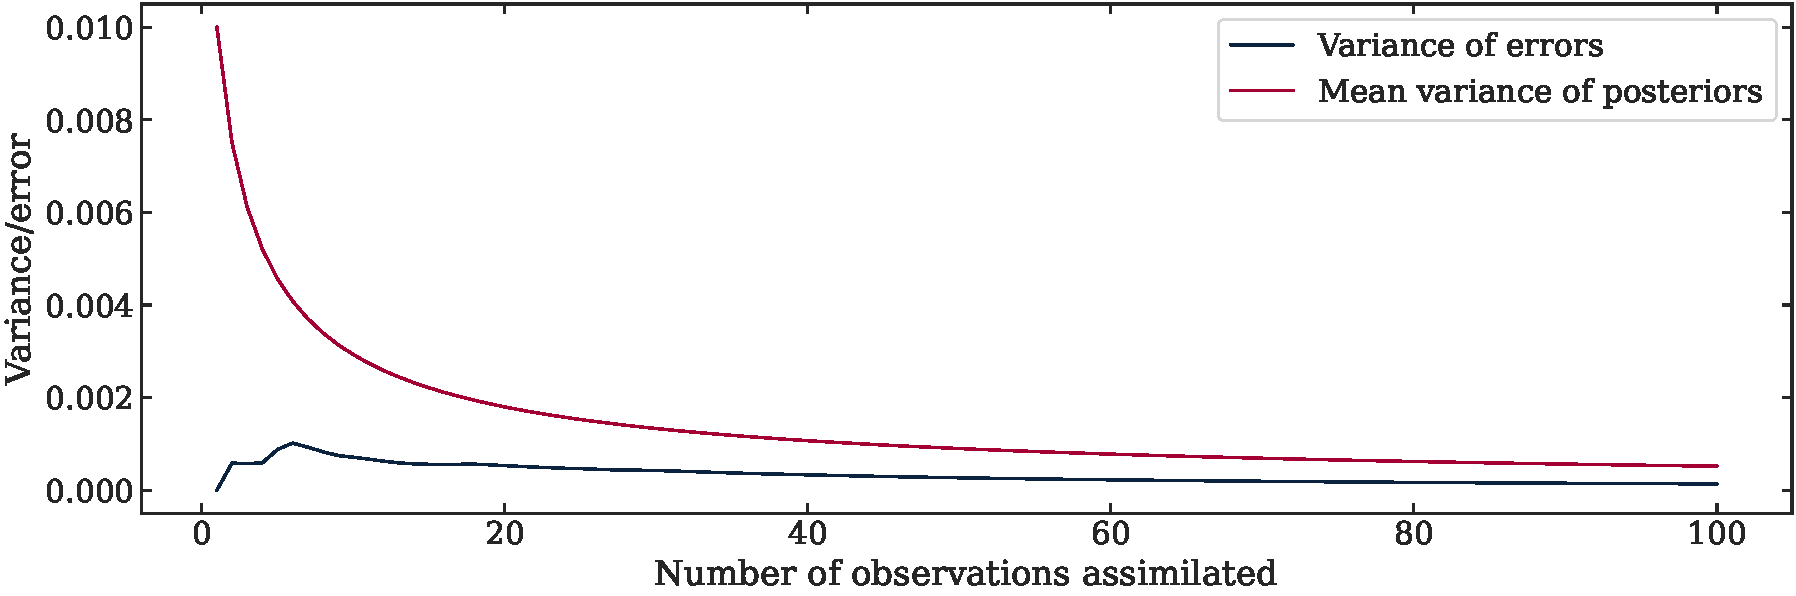
\includegraphics[width=\textwidth]{figures/stats_point1_var01.pdf}
      \subcaption{$\sigma_y^2 = \qty{0.01}{m^2}$}
   \end{subfigure}

   \caption{Evolution of statistics for assimilation of 100 observations at Point 1 (\ang{40} N).}
\end{figure}

After about 20 observations, the variances of the prior and posterior error are essentially identical and continue to decrease together. The prior error lags behind the posterior error by one observation. The decay rate of the error variance appears independent of the observation variance, only the magnitude differs by $\num{e3}$, which corresponds to the change in observation variance from \qty{10}{m^2} to \qty{0.01}{m^2}.

The reason for the convergence of prior and posterior error is in the definition of the gain $K = \sigma_p^2 / (\sigma_p^2 + \sigma_y^2)$. The prior variance $\sigma_p^2$ shrinks with every observation because $0 < K < 1$ for a non-zero observation variance $\sigma_y^2$. As $\sigma_p^2 \to 0$, the gain $K \to 0$ and therefore the posterior does not change much compared to the prior.



\section{Single scalar observations for other point}

\begin{figure}[H]
   \centering
   
   \begin{subfigure}[c]{0.8\textwidth}
      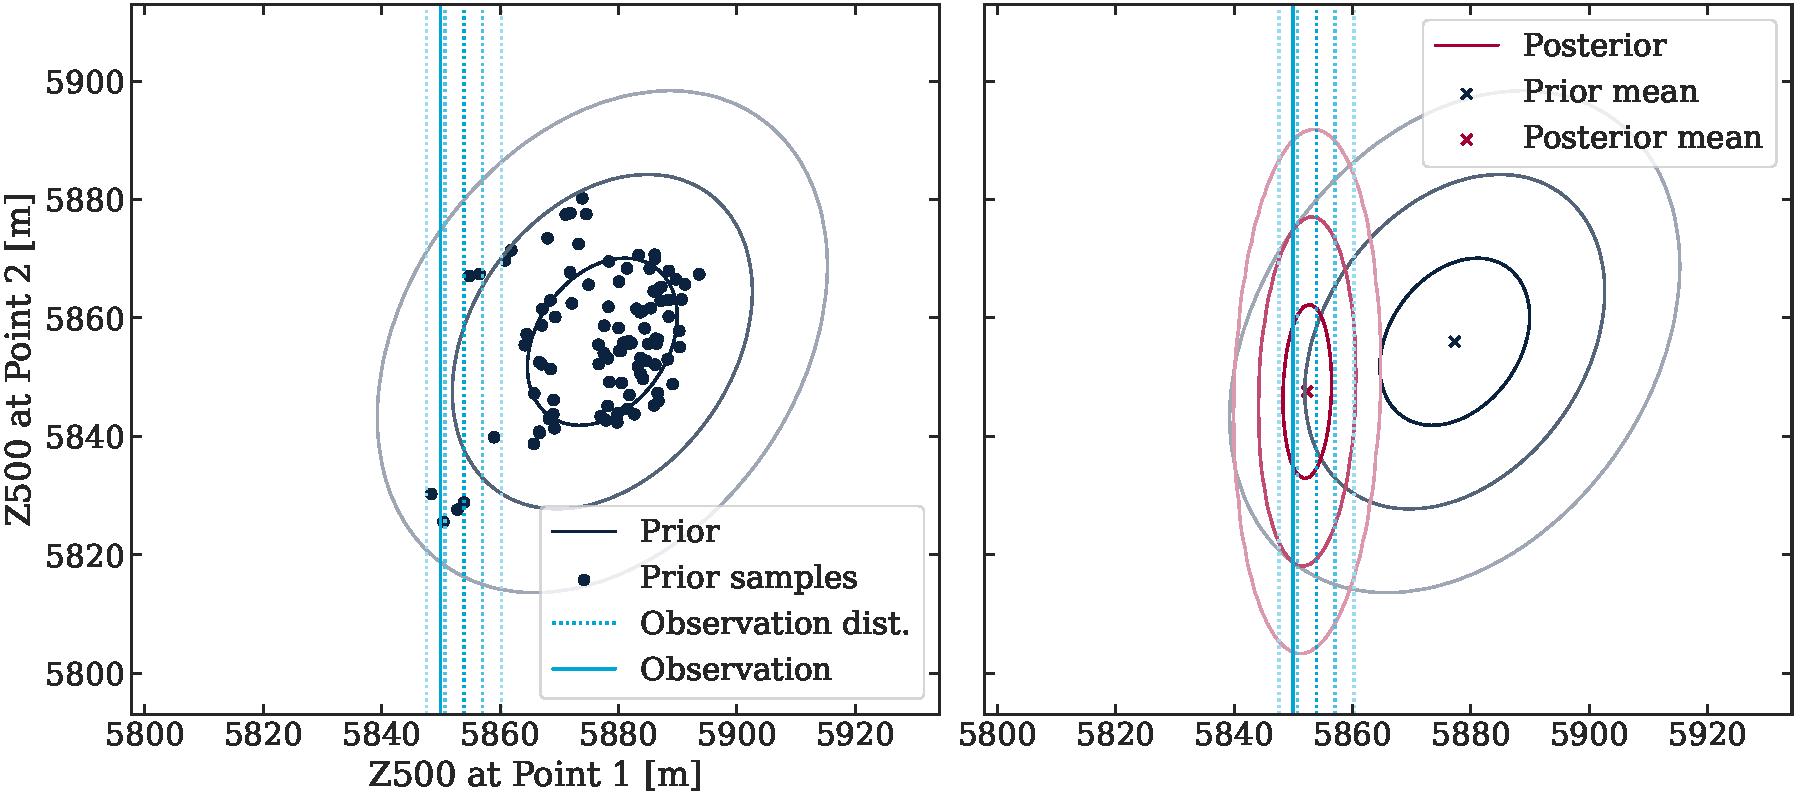
\includegraphics[width=\textwidth]{figures/vector_1.pdf}
      \subcaption{Observation at Point 1 (\ang{40} N)}
      \label{fig:vector-1}
   \end{subfigure}
   
   \bigskip
   
   \begin{subfigure}[c]{0.8\textwidth}
      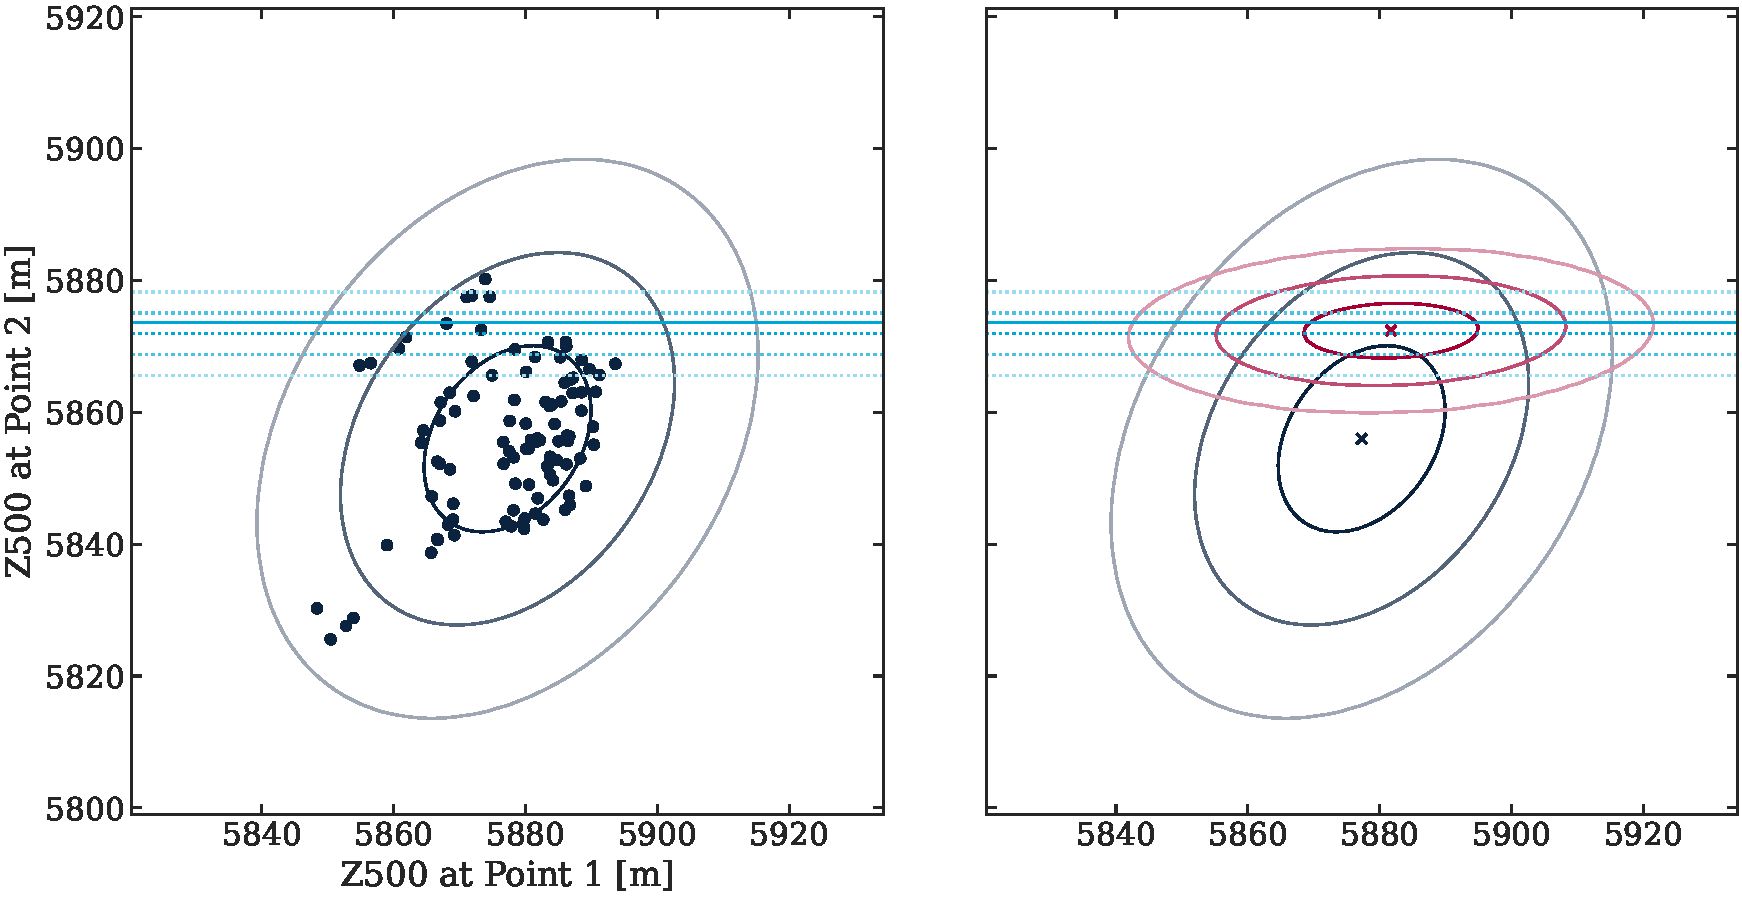
\includegraphics[width=\textwidth]{figures/vector_2.pdf}
      \subcaption{Observation at Point 2 (\ang{20} N)}
      \label{fig:vector-2}
   \end{subfigure}

   \caption{Assimilation of a single scalar observation with a joint state. Contours and vertical lines indicate constant probability density at 1-$\sigma$ intervals.}
\end{figure}



I will only discuss \cref{fig:vector-1}, but results for \cref{fig:vector-2} are analogous.

To update both points with an observation at point 1, the observation matrix is $H = \smqty[1 & 0]$ and the observation covariance matrix is $R = \smqty[\qty{10}{m^2}]$. The Kalman gain matrix takes care of propagating the information to point 2 via the prior covariance matrix.

After assimilating the observation for point 1, the variance of Z500 at point 1 shrinks from \qty{104}{m^2} to \qty{9}{m^2}. For point 2, the variance reduces from \qty{130}{m^2} to \qty{119}{m^2}. The mean shifts by \qty{25}{m} for point 1 and by \qty{8}{m} for point 2. Point 1 benefits much more from observations at point 1, as expected. Still, point 2 is updated appreciably, mediated by the prior covariance (off-diagonal element) of \qty{35}{m^2}.

I would have expected have expected the update of the unobserved point to be strictly along the major axis of the prior covariance ellipse (i.e., along its first principal component), which is not the case. Also, I would have expected the variance of point 2 to decrease more.




\end{document}
